%
% file: localoperator.tex
% author: Victor Brena
% description: Briefly describes properties of the local operator.
%

\chapter{Appendix A}\label{app:app01}
\section*{Two Way Ranging (TWR)} % TODO: Look at pulling this put into an appendix?
TWR is a ranging method that utilises TOF and delays during transmission of a packet in order to determine the range between a tag and anchor.
Figure~\ref{fig:twr} provides a simple illustration of how this works.
The distance for an individual tag and an anchor can be obtained by:
\[
    d=c.\frac{(TT2-TT1)-(TA2-TA2)}{2}
\]
This is repeated for each anchor and then the position of the tag can be determined via trilateration.
Geometrically, the position of the tag can be described as the point intersection of all the circles with distance,d , from the tag.
This can be seen in Figure~\ref{fig:trilat}.
\begin{figure}[h!]
    \centering
    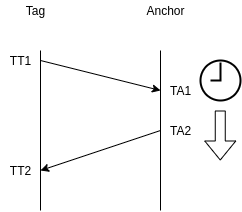
\includegraphics[scale=.7]{lr/TWR}
    \caption{Packet transfer in TWR.}
    \label{fig:twr}
\end{figure}

\begin{figure}[h!]
    \centering
    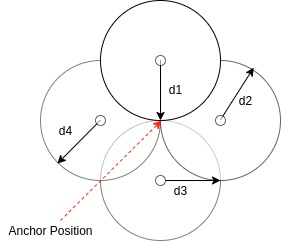
\includegraphics[scale=.7]{lr/trilat}
    \caption{4 Anchor and 1 Tag trilateration in 2D.}
    \label{fig:trilat}
\end{figure}
\newpage










